
\section{Higher Order Runge Kutta Methods}
\label{section:HBs_and_higher_order_RK}
In this section, we attempt to perform defect control based on efficient multistep interpolants for higher order Runge-Kutta methods. We recall that related previous work used significantly more stages to obtain a continuous $6^{th}$ order Runge-Kutta method and a continuous $8^{th}$ order Runge-Kutta method.

In this section, we will first augment the RK6 method (see Section $\ref{section:basic_runge_kutta}$ for details about the discrete method) with HB6 and then with HB8. We hope to perform defect control and to find that the use of HB8 allows significantly fewer steps. We will then augment the RK8 method (see Section $\ref{section:basic_runge_kutta}$ for more details) with HB8 to show that though interpolation error is present, the scheme does allow defect control of a continuous $8^{th}$ order solution. 

For both methods, we will sample the defect only twice in a step, at $0.4h$ and $0.8h$ in a step of size $h$, as the previous experiments appears to indicate that the maximum defects tend to occur at these locations within each step.

\subsection{RK6 with HB6}
\paragraph{Problem 1 results}
Figures $\ref{fig:rk6_with_hb6_p1_global_defect}$, $\ref{fig:rk6_with_hb6_p1_global_error}$ and $\ref{fig:rk6_with_hb6_p1_scaled_defects}$ shows the results of using RK6 with HB6 on Problem 1. We note that an absolute tolerance of $10^{-6}$ is applied on the maximum defect within the step and this can be shown to occur at $0.3h$ and $0.8h$ along a step of size, h. See Figure $\ref{fig:rk6_with_hb6_p1_scaled_defects}$, to see the scaled defect reaching a maximum near these points. We note that we are able to successfully control the defect of the continuous numerical solution using this approach, see Figure $\ref{fig:rk6_with_hb6_p1_global_defect}$. 

\begin{figure}[H]
\centering
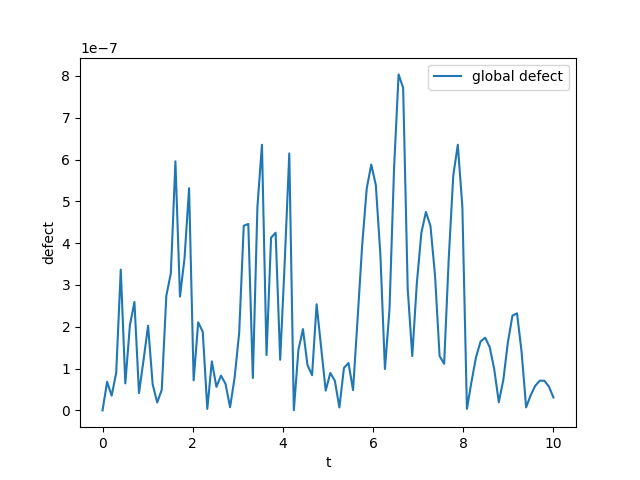
\includegraphics[width=0.7\linewidth]{./figures/rk6_with_hb6_p1_global_defect}
\caption{Defect across the entire domain for RK6 with HB6 on problem 1 at an absolute tolerance of $10^{-6}$.}
\label{fig:rk6_with_hb6_p1_global_defect}
\end{figure}

\begin{figure}[H]
\centering
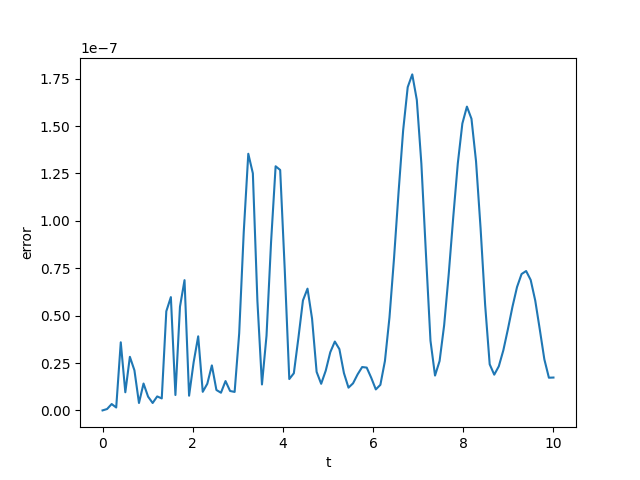
\includegraphics[width=0.7\linewidth]{./figures/rk6_with_hb6_p1_global_error}
\caption{Global Error for RK6 with HB6 on problem 1 at an absolute tolerance of $10^{-6}$.}
\label{fig:rk6_with_hb6_p1_global_error}
\end{figure}

\begin{figure}[H]
\centering
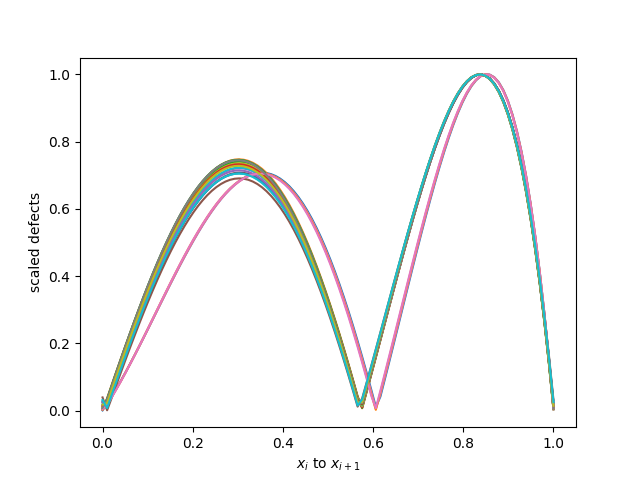
\includegraphics[width=0.7\linewidth]{./figures/rk6_with_hb6_p1_scaled_defects}
\caption{Scaled defects for RK6 with HB6 on problem 1 at an absolute tolerance of $10^{-6}$ mapped onto $[0, 1]$.}
\label{fig:rk6_with_hb6_p1_scaled_defects}
\end{figure}

\paragraph{Problem 2 results}
Figures $\ref{fig:rk6_with_hb6_p2_global_defect}$, $\ref{fig:rk6_with_hb6_p2_global_error}$ and $\ref{fig:rk6_with_hb6_p2_scaled_defects}$ shows the results of using RK6 with HB6 on Problem 2. We note that an absolute tolerance of $10^{-6}$ is applied on the maximum defect within the step and this can be shown to occur at $0.3h$ or $0.8h$ along a step of size, h. See Figure $\ref{fig:rk6_with_hb6_p2_scaled_defects}$, to see the scaled defect reaching a maximum near these points. We note that we are able to successfully control the defect of the continuous numerical solution using this approach, see Figure $\ref{fig:rk6_with_hb6_p2_global_defect}$. 

\begin{figure}[H]
\centering
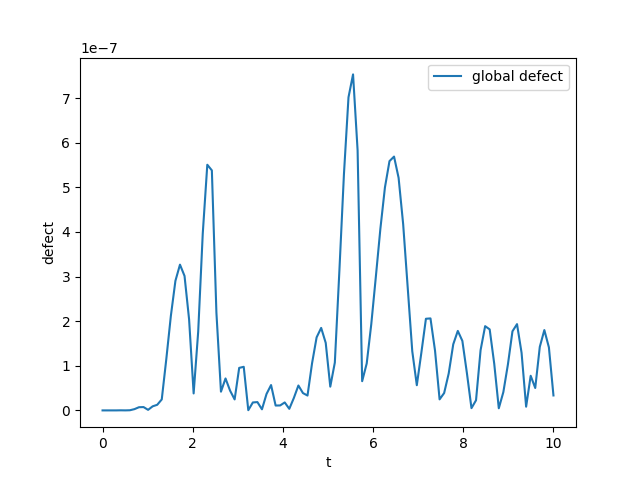
\includegraphics[width=0.7\linewidth]{./figures/rk6_with_hb6_p2_global_defect}
\caption{Defect across the entire domain for RK6 with HB6 on problem 2 at an absolute tolerance of $10^{-6}$.}
\label{fig:rk6_with_hb6_p2_global_defect}
\end{figure}

\begin{figure}[H]
\centering
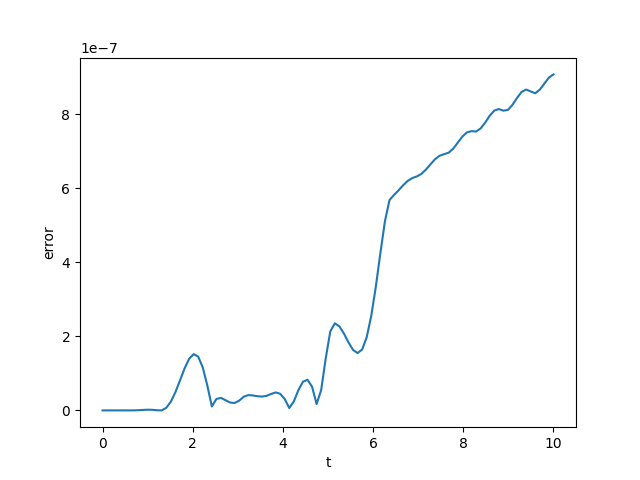
\includegraphics[width=0.7\linewidth]{./figures/rk6_with_hb6_p2_global_error}
\caption{Global Error for RK6 with HB6 on problem 2 at an absolute tolerance of $10^{-6}$.}
\label{fig:rk6_with_hb6_p2_global_error}
\end{figure}

\begin{figure}[H]
\centering
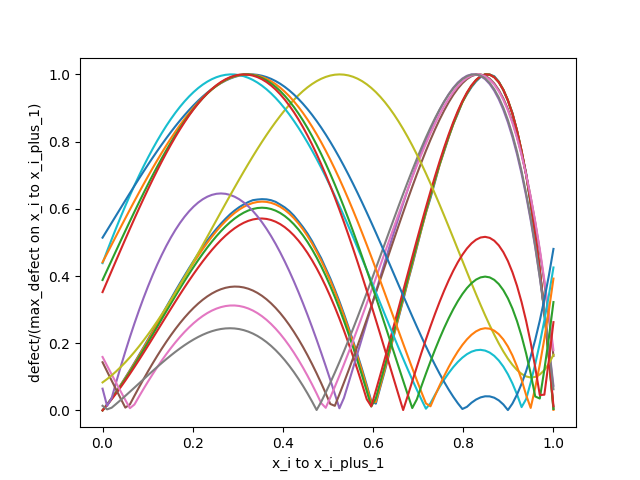
\includegraphics[width=0.7\linewidth]{./figures/rk6_with_hb6_p2_scaled_defects}
\caption{Scaled defects for RK6 with HB6 on problem 2 at an absolute tolerance of $10^{-6}$ mapped onto $[0, 1]$.}
\label{fig:rk6_with_hb6_p2_scaled_defects}
\end{figure}

\begin{figure}[H]
\centering
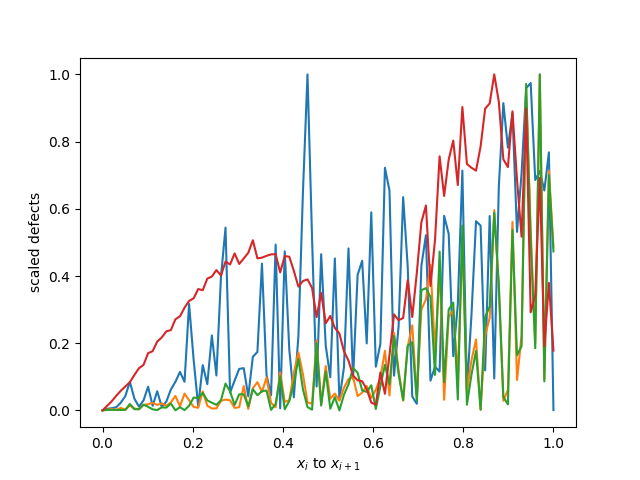
\includegraphics[width=0.7\linewidth]{./figures/rk6_with_hb6_p2_scaled_defects_small_steps}
\caption{Scaled defects for RK6 with HB6 on small steps on problem 2 at an absolute tolerance of $10^{-6}$ mapped onto $[0, 1]$. Despite the noise, for most steps, the maximum defect mostly appears near $0.8h$.}
\label{fig:rk6_with_hb6_p2_scaled_defects_small_steps}
\end{figure}

\paragraph{Problem 3 results}
Figures $\ref{fig:rk6_with_hb6_p3_global_defect}$, $\ref{fig:rk6_with_hb6_p3_global_error}$ and $\ref{fig:rk6_with_hb6_p3_scaled_defects}$ shows the results of using RK6 with HB6 on Problem 3. 
We note that an absolute tolerance of $10^{-6}$ is applied on the maximum defect within the step and this can be shown to occur at $0.3h$ or $0.8h$ along a step of size, h. See Figure $\ref{fig:rk6_with_hb6_p3_scaled_defects}$, to see the scaled defect reaching a maximum near these points. We note that we are able to successfully control the defect of the continuous numerical solution using this approach, see Figure $\ref{fig:rk6_with_hb6_p3_global_defect}$. 

\begin{figure}[H]
\centering
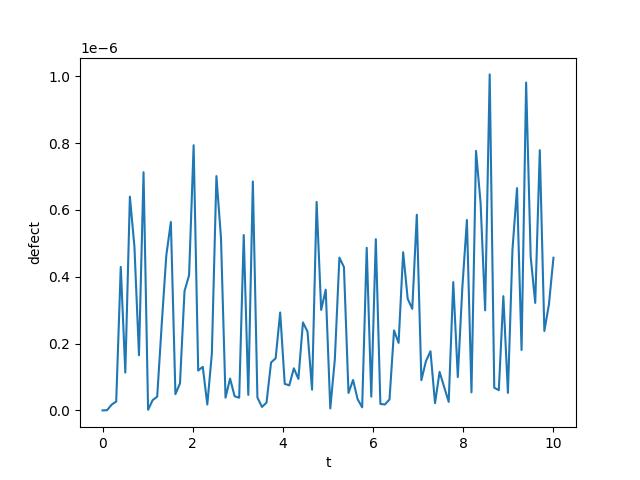
\includegraphics[width=0.7\linewidth]{./figures/rk6_with_hb6_p3_global_defect}
\caption{Defect across the entire domain for RK6 with HB6 on problem 3 at an absolute tolerance of $10^{-6}$.}
\label{fig:rk6_with_hb6_p3_global_defect}
\end{figure}

\begin{figure}[H]
\centering
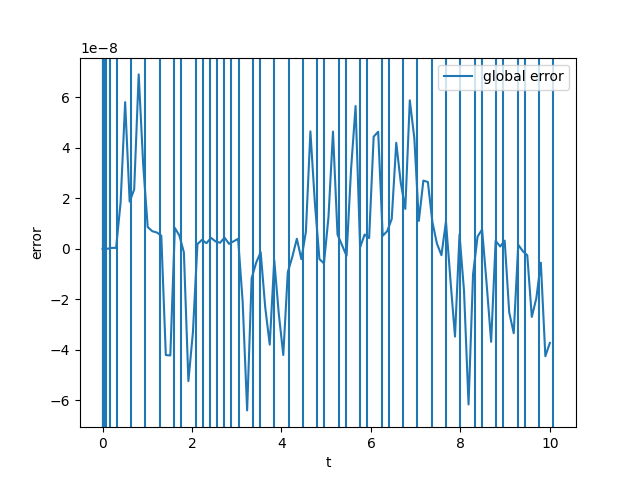
\includegraphics[width=0.7\linewidth]{./figures/rk6_with_hb6_p3_global_error}
\caption{Global Error for RK6 with HB6 on problem 3 at an absolute tolerance of $10^{-6}$.}
\label{fig:rk6_with_hb6_p3_global_error}
\end{figure}

\begin{figure}[H]
\centering
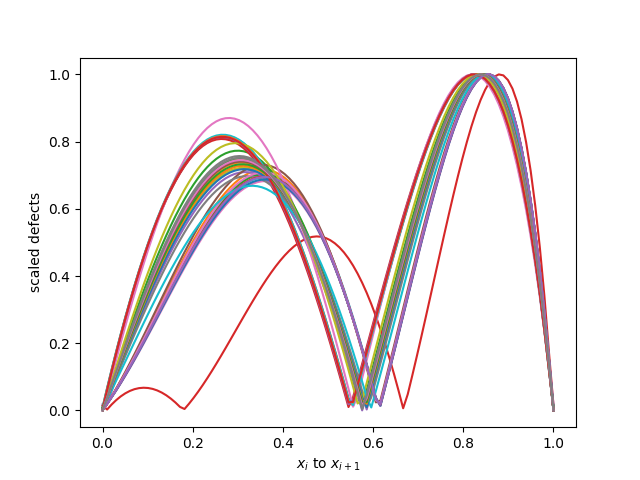
\includegraphics[width=0.7\linewidth]{./figures/rk6_with_hb6_p3_scaled_defects}
\caption{Scaled defects for RK6 with HB6 on problem 3 at an absolute tolerance of $10^{-6}$ mapped onto $[0, 1]$.}
\label{fig:rk6_with_hb6_p3_scaled_defects}
\end{figure}

\begin{figure}[H]
\centering
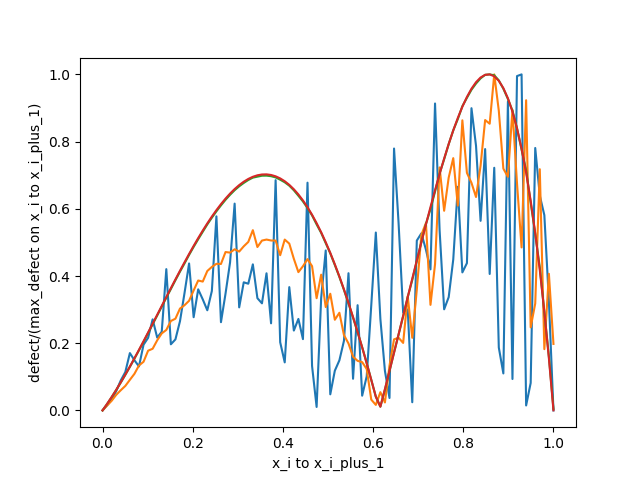
\includegraphics[width=0.7\linewidth]{./figures/rk6_with_hb6_p3_scaled_defects_small_steps}
\caption{Scaled defects for RK6 with HB6 on small steps on problem 3 at an absolute tolerance of $10^{-6}$ mapped onto $[0, 1]$.}
\label{fig:rk6_with_hb6_p3_scaled_defects_small_steps}
\end{figure}

\subsection{RK6 with HB8}
\paragraph{Problem 1 results}
Figures $\ref{fig:rk6_with_hb8_p1_global_defect}$, $\ref{fig:rk6_with_hb8_p1_global_error}$ and $\ref{fig:rk6_with_hb8_p1_scaled_defects}$ shows the results of using RK6 with HB8 on Problem 1. We note that an absolute tolerance of $10^{-6}$ is applied on the maximum defect within the step and this can be shown to occur at $0.4h$ and $0.8h$ along a step of size, h. See Figure $\ref{fig:rk6_with_hb8_p1_scaled_defects}$, to see the scaled defect reaching a maximum near these points. We note that we are able to successfully control the defect of the continuous numerical solution using this approach, see Figure $\ref{fig:rk6_with_hb8_p1_global_defect}$. 


\begin{figure}[H]
\centering
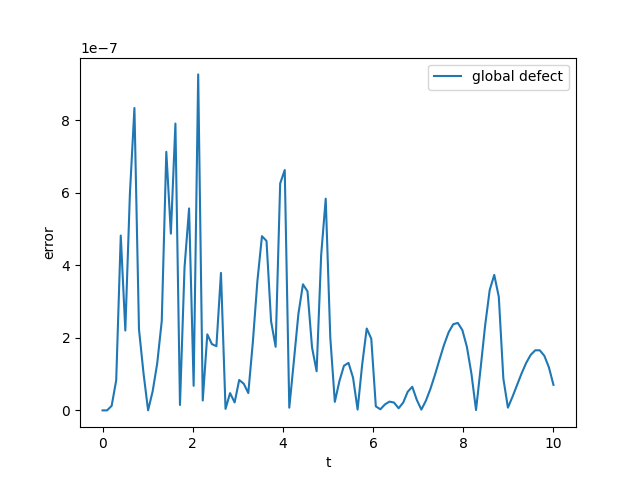
\includegraphics[width=0.7\linewidth]{./figures/rk6_with_hb8_p1_global_defect}
\caption{Defect across the entire domain for RK6 with HB8 on problem 1 at an absolute tolerance of $10^{-6}$.}
\label{fig:rk6_with_hb8_p1_global_defect}
\end{figure}

\begin{figure}[H]
\centering
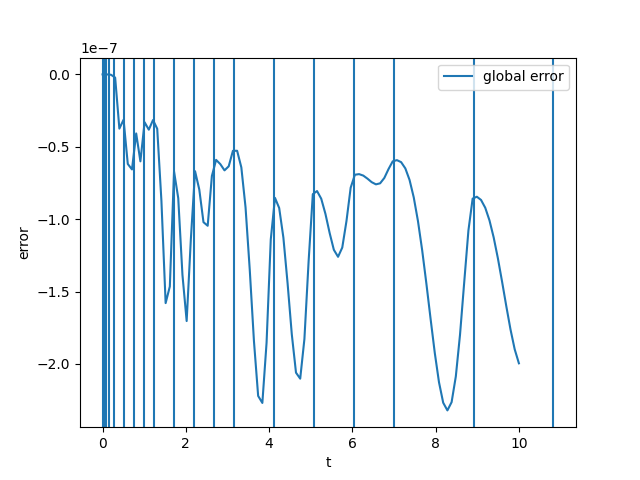
\includegraphics[width=0.7\linewidth]{./figures/rk6_with_hb8_p1_global_error}
\caption{Global Error for RK6 with HB8 on problem 1 at an absolute tolerance of $10^{-6}$.}
\label{fig:rk6_with_hb8_p1_global_error}
\end{figure}

\begin{figure}[H]
\centering
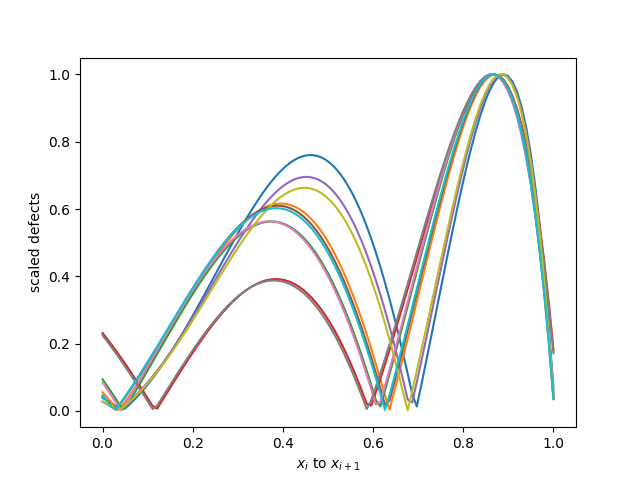
\includegraphics[width=0.7\linewidth]{./figures/rk6_with_hb8_p1_scaled_defects}
\caption{Scaled defects for RK6 with HB8 on problem 1 at an absolute tolerance of $10^{-6}$ mapped onto $[0, 1]$.}
\label{fig:rk6_with_hb8_p1_scaled_defects}
\end{figure}

\paragraph{Problem 2 results}
Figures $\ref{fig:rk6_with_hb8_p2_global_defect}$, $\ref{fig:rk6_with_hb8_p2_global_error}$ and $\ref{fig:rk6_with_hb8_p2_scaled_defects}$ shows the results of using RK6 with HB8 on Problem 2. We note that an absolute tolerance of $10^{-6}$ is applied on the maximum defect within the step and this can be shown to occur at $0.8h$ along a step of size, h. See Figure $\ref{fig:rk6_with_hb8_p2_scaled_defects}$, to see the scaled defect reaching a maximum near these points. We note that we are able to successfully control the defect of the continuous numerical solution using this approach, see Figure $\ref{fig:rk6_with_hb8_p2_global_defect}$. 


\begin{figure}[H]
\centering
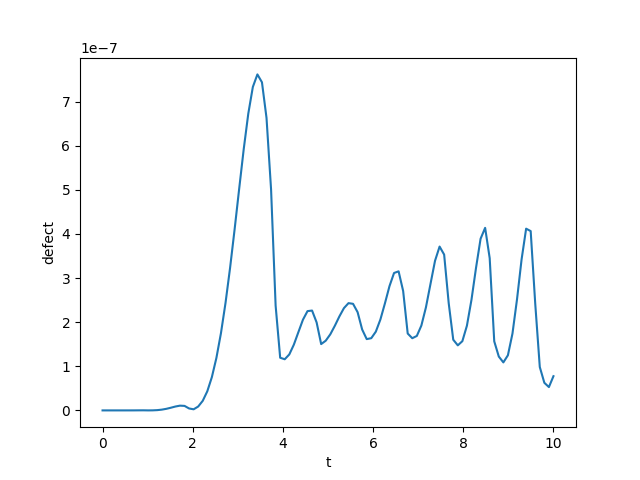
\includegraphics[width=0.7\linewidth]{./figures/rk6_with_hb8_p2_global_defect}
\caption{Defect across the entire domain for RK6 with HB8 on problem 2 at an absolute tolerance of $10^{-6}$.}
\label{fig:rk6_with_hb8_p2_global_defect}
\end{figure}

\begin{figure}[H]
\centering
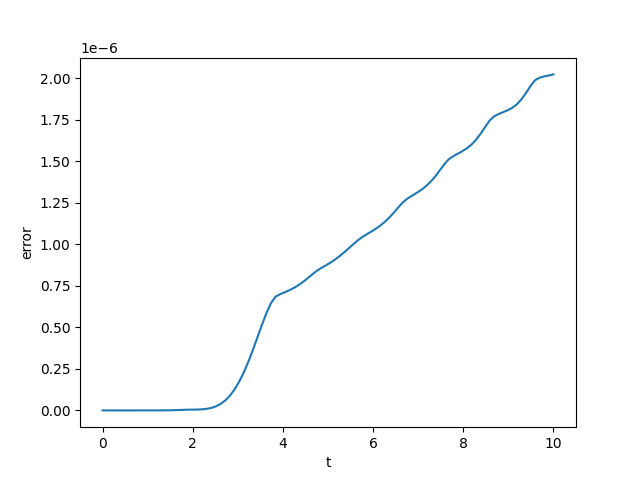
\includegraphics[width=0.7\linewidth]{./figures/rk6_with_hb8_p2_global_error}
\caption{Global Error for RK6 with HB8 on problem 2 at an absolute tolerance of $10^{-6}$.}
\label{fig:rk6_with_hb8_p2_global_error}
\end{figure}

\begin{figure}[H]
\centering
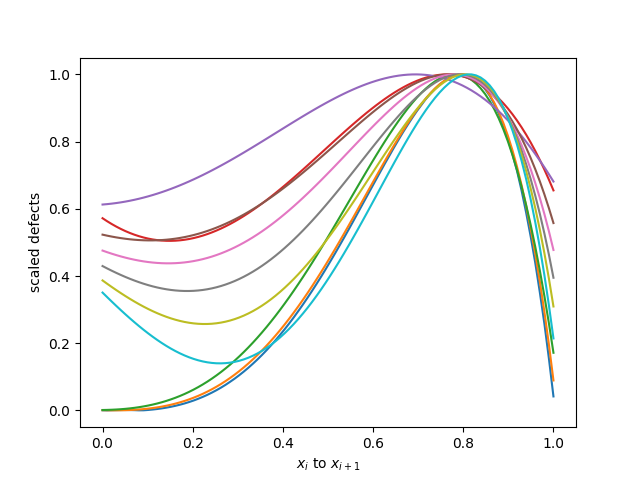
\includegraphics[width=0.7\linewidth]{./figures/rk6_with_hb8_p2_scaled_defects}
\caption{Scaled defects for RK6 with HB8 on problem 2 at an absolute tolerance of $10^{-6}$ mapped onto $[0, 1]$.}
\label{fig:rk6_with_hb8_p2_scaled_defects}
\end{figure}

\begin{figure}[H]
\centering
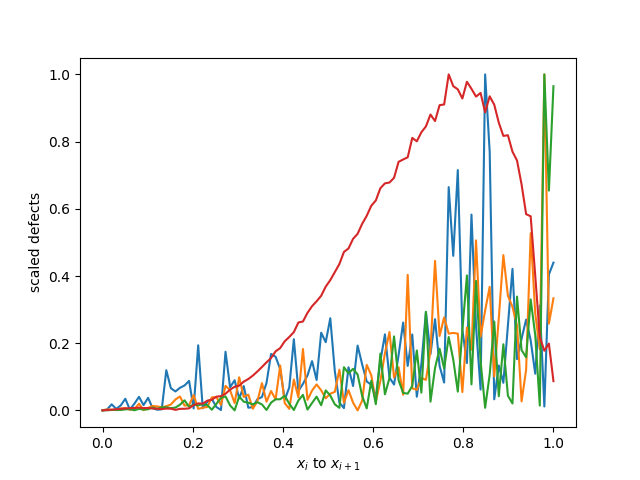
\includegraphics[width=0.7\linewidth]{./figures/rk6_with_hb8_p2_scaled_defects_small_steps}
\caption{Scaled defects for RK6 with HB8 on small steps on problem 2 at an absolute tolerance of $10^{-6}$ mapped onto $[0, 1]$. Despite the noise, the maximum defect mostly appears near $0.8h$.}
\label{fig:rk6_with_hb8_p2_scaled_defects_small_steps}
\end{figure}

\paragraph{Problem 3 results}
Figures $\ref{fig:rk6_with_hb8_p3_global_defect}$, $\ref{fig:rk6_with_hb8_p3_global_error}$ and $\ref{fig:rk6_with_hb8_p3_scaled_defects}$ shows the results of RK6 with HB8 on Problem 3. 
We note that an absolute tolerance of $10^{-6}$ is applied on the maximum defect within the step and this can be shown to occur at either $0.4h$ or $0.8h$ along a step of size, h. See Figure $\ref{fig:rk6_with_hb8_p3_scaled_defects}$, to see the scaled defect reaching a maximum near these points. We note that we are able to successfully control the defect of the continuous numerical solution using this approach, see Figure $\ref{fig:rk6_with_hb8_p3_global_defect}$. 
 

\begin{figure}[H]
\centering
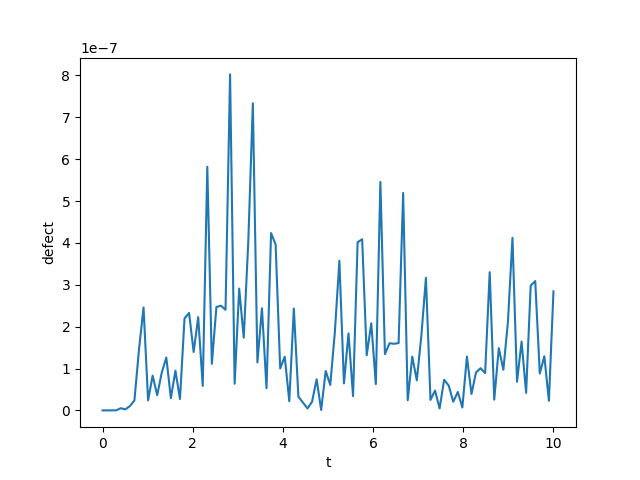
\includegraphics[width=0.7\linewidth]{./figures/rk6_with_hb8_p3_global_defect}
\caption{Defect across the entire domain for RK6 with HB8 on problem 3 at an absolute tolerance of $10^{-6}$.}
\label{fig:rk6_with_hb8_p3_global_defect}
\end{figure}

\begin{figure}[H]
\centering
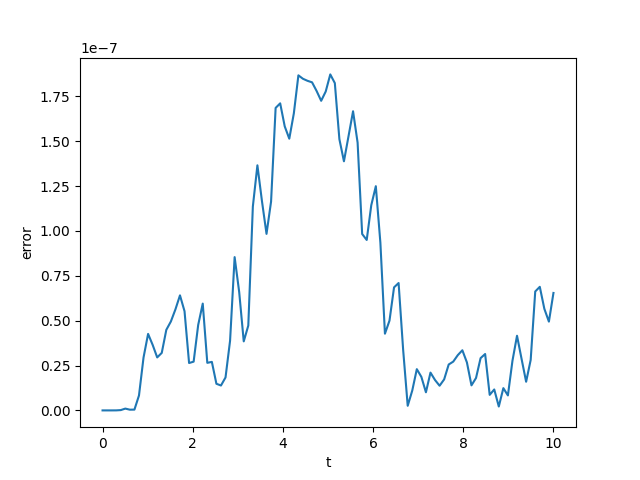
\includegraphics[width=0.7\linewidth]{./figures/rk6_with_hb8_p3_global_error}
\caption{Global Error for RK6 with HB8 on problem 3 at an absolute tolerance of $10^{-6}$.}
\label{fig:rk6_with_hb8_p3_global_error}
\end{figure}

\begin{figure}[H]
\centering
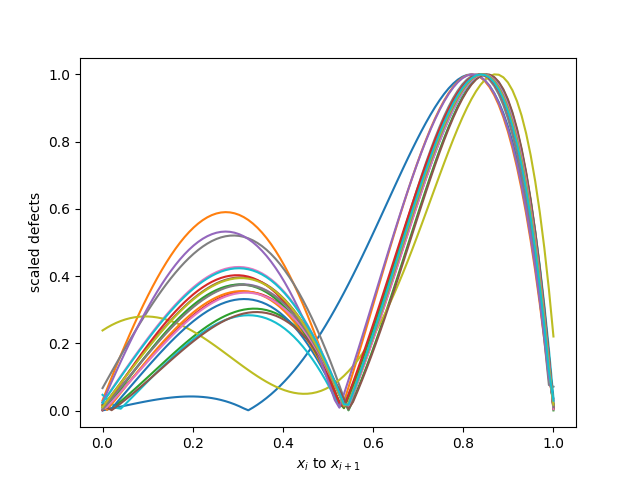
\includegraphics[width=0.7\linewidth]{./figures/rk6_with_hb8_p3_scaled_defects}
\caption{Scaled defects for RK6 with HB8 on problem 3 at an absolute tolerance of $10^{-6}$ mapped onto $[0, 1]$.}
\label{fig:rk6_with_hb8_p3_scaled_defects}
\end{figure}

\begin{figure}[H]
\centering
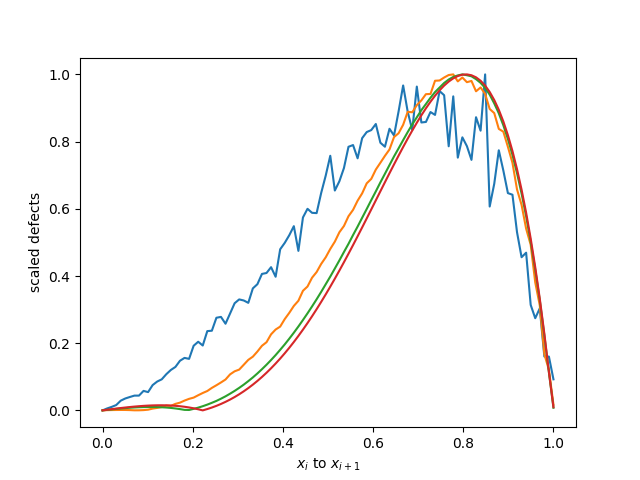
\includegraphics[width=0.7\linewidth]{./figures/rk6_with_hb8_p3_scaled_defects_small_steps}
\caption{Scaled defects for RK6 with HB8 on small steps on problem 3 at an absolute tolerance of $10^{-6}$ mapped onto $[0, 1]$. Despite the noise, the maximum defect mostly appears near $0.8h$.}
\label{fig:rk6_with_hb8_p3_scaled_defects_small_steps}
\end{figure}

\begin{table}[h]
\caption {Number of steps taken by RK6 when modified to do defect control with HB8 vs when modified with HB6.} \label{tab:rk6_with_hb6_vs_hb8_nsteps}
\begin{center}
\begin{tabular}{ c c c c c } 
Problem & succ. steps HB8 & succ. steps HB6 & nsteps HB8 & nsteps HB6 \\ 
1       & 18                 &        26          & 18         & 27\\ 
2       & 14                 &        18          & 17         & 23\\
3       & 24                 &        42          & 26         & 51\\
\end{tabular}
\end{center}
\end{table}

From Table $\ref{tab:rk6_with_hb6_vs_hb8_nsteps}$, we can see that again, using an interpolant whose interpolation error and especially the interpolation error of its derivative is of higher order than the ODE solution drastically reduces the number of steps. The solver becomes more efficient as a result. Since RK6 with HB6 and with HB8 is behaving similarly to RK4 with HB4 and with HB6, we expect that using a $10^{th}$ order method would not improve the situation more than HB8 has over HB6. Though fitting RK6 with HB10 will be as efficient as fitting it with HB8, the fact that the interpolation error is no longer the limiting factor means that HB10 will not improve the situation. For RK6, HB8 is the preferred interpolant.  

We also note that during the solving of the 3 problems, the value of $\alpha$ with HB6 rarely was bigger than 4 or smaller than $\frac{1}{4}$. The values of $\alpha$ and $\beta$ with HB8 also rarely were bigger than 4 or smaller than $\frac{1}{4}$. 

\subsection{RK8 with HB8}
In this section, we fit the RK8 method, described in Section $\ref{section:basic_runge_kutta}$, with HB8. Though we expect the interpolation error to reduce the efficiency of this scheme, we provide a proof of concept that an RK8 can have defect control with the scheme presented in this chapter. We will look into the challenges and possibilities of deriving an HB10 scheme in the Future Work section. 

\paragraph{Problem 1 results}
Figures $\ref{fig:rk8_with_hb8_p1_global_defect}$, $\ref{fig:rk8_with_hb8_p1_global_error}$ and $\ref{fig:rk8_with_hb8_p1_scaled_defects}$ shows the results of using RK8 with HB8 on Problem 1. We note that an absolute tolerance of $10^{-6}$ is applied on the maximum defect within the step and this can be shown to occur at $0.3h$ and $0.8h$ along a step of size, h. See Figure $\ref{fig:rk8_with_hb8_p1_scaled_defects}$, to see the scaled defect reaching a maximum near these points. We note that we are able to successfully control the defect of the continuous numerical solution using this approach, see Figure $\ref{fig:rk8_with_hb8_p1_global_defect}$. 
 

\begin{figure}[H]
\centering
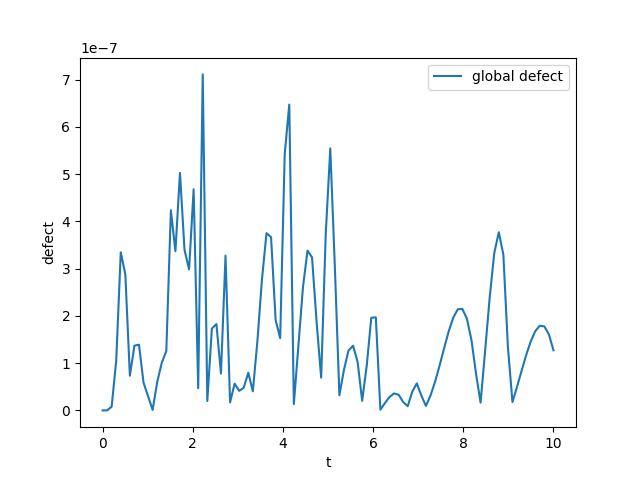
\includegraphics[width=0.7\linewidth]{./figures/rk8_with_hb8_p1_global_defect}
\caption{Defect across the entire domain for RK8 with HB8 on problem 1 at an absolute tolerance of $10^{-6}$.}
\label{fig:rk8_with_hb8_p1_global_defect}
\end{figure}

\begin{figure}[H]
\centering
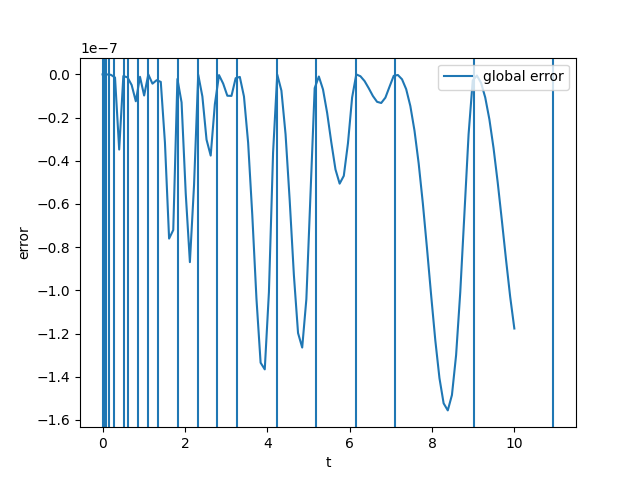
\includegraphics[width=0.7\linewidth]{./figures/rk8_with_hb8_p1_global_error}
\caption{Global Error for RK8 with HB8 on problem 1 at an absolute tolerance of $10^{-6}$.}
\label{fig:rk8_with_hb8_p1_global_error}
\end{figure}

\begin{figure}[H]
\centering
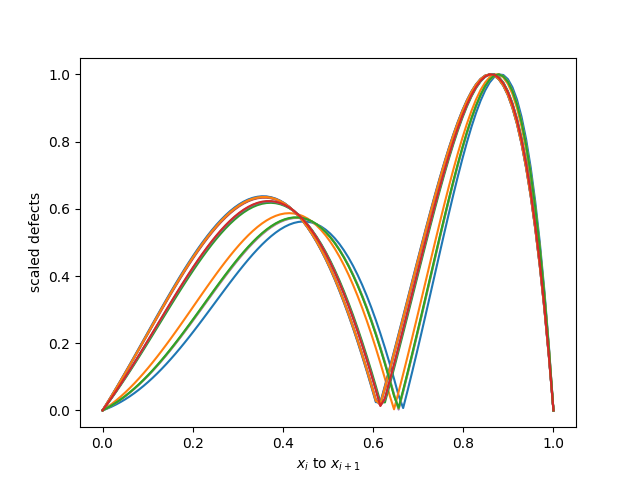
\includegraphics[width=0.7\linewidth]{./figures/rk8_with_hb8_p1_scaled_defects}
\caption{Scaled defects for RK8 with HB8 on problem 1 at an absolute tolerance of $10^{-6}$  mapped onto $[0, 1]$.}
\label{fig:rk8_with_hb8_p1_scaled_defects}
\end{figure}

\paragraph{Problem 2 results}
Figures $\ref{fig:rk8_with_hb8_p2_global_defect}$, $\ref{fig:rk8_with_hb8_p2_global_error}$ and $\ref{fig:rk8_with_hb8_p2_scaled_defects}$ shows the results of using RK8 with HB8 on Problem 2. We note that an absolute tolerance of $10^{-6}$ is applied on the maximum defect within the step and this can be shown to occur at $0.3h$ or $0.8h$ along a step of size, h. See Figure $\ref{fig:rk8_with_hb8_p2_scaled_defects}$, to see the scaled defect reaching a maximum near these points. We note that we are able to successfully control the defect of the continuous numerical solution using this approach, see Figure $\ref{fig:rk8_with_hb8_p2_global_defect}$. 

\begin{figure}[H]
\centering
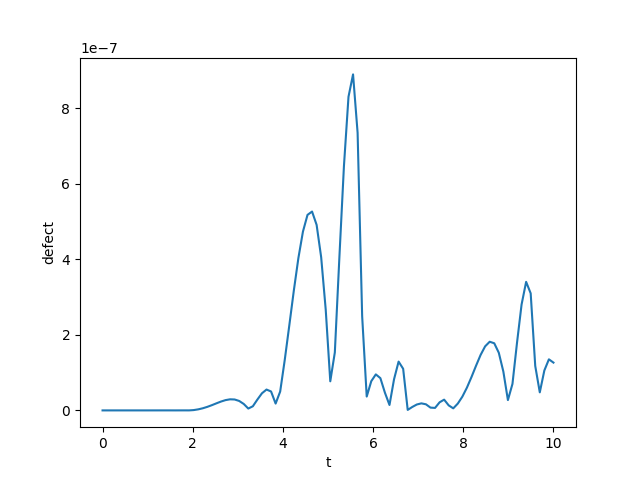
\includegraphics[width=0.7\linewidth]{./figures/rk8_with_hb8_p2_global_defect}
\caption{Defect across the entire domain for RK8 with HB8 on problem 2 at an absolute tolerance of $10^{-6}$.}
\label{fig:rk8_with_hb8_p2_global_defect}
\end{figure}

\begin{figure}[H]
\centering
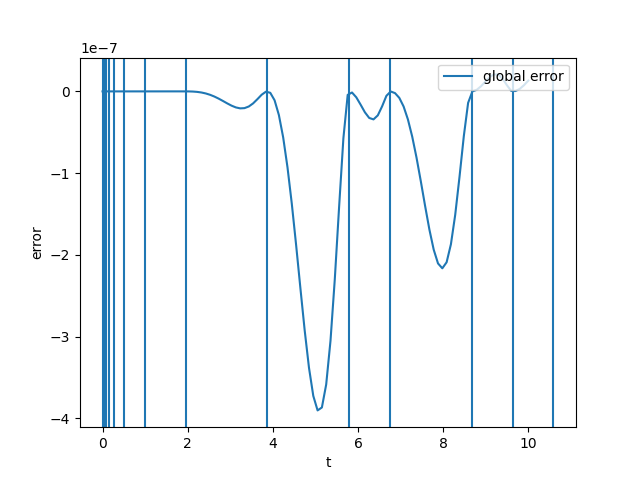
\includegraphics[width=0.7\linewidth]{./figures/rk8_with_hb8_p2_global_error}
\caption{Global Error for RK8 with HB8 on problem 2 at an absolute tolerance of $10^{-6}$.}
\label{fig:rk8_with_hb8_p2_global_error}
\end{figure}

\begin{figure}[H]
\centering
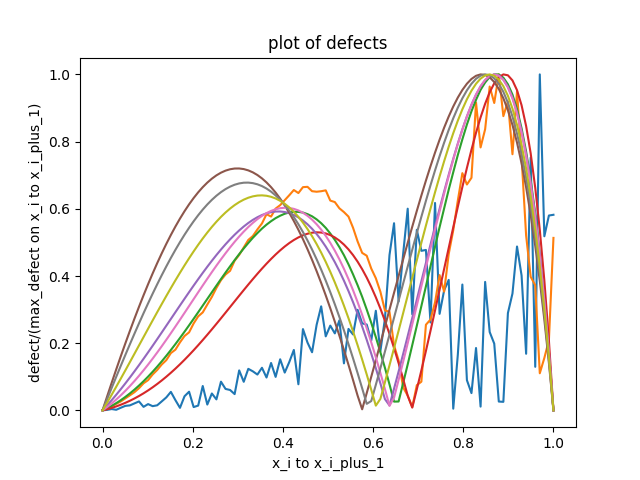
\includegraphics[width=0.7\linewidth]{./figures/rk8_with_hb8_p2_scaled_defects}
\caption{Scaled defects for RK8 with HB8 on problem 2 at an absolute tolerance of $10^{-6}$  mapped onto $[0, 1]$.}
\label{fig:rk8_with_hb8_p2_scaled_defects}
\end{figure}

\begin{figure}[H]
\centering
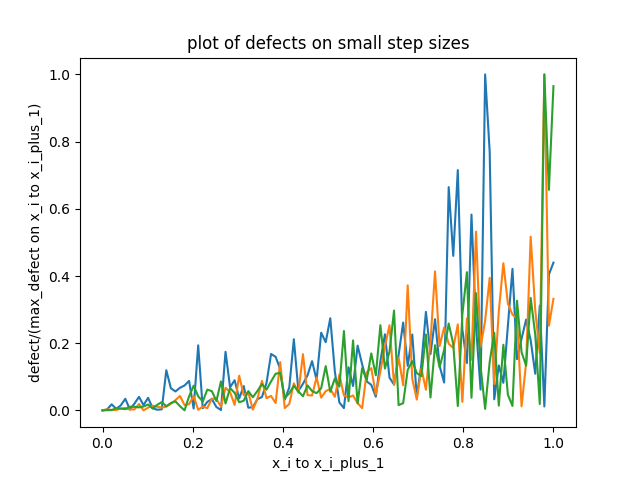
\includegraphics[width=0.7\linewidth]{./figures/rk8_with_hb8_p2_scaled_defects_small_steps}
\caption{Scaled defects of RK8 with HB8 on small steps on problem 2 at an absolute tolerance of $10^{-6}$ mapped onto $[0, 1]$. Despite the noise, the maximum defect mostly appears near $0.8h$.}
\label{fig:rk8_with_hb8_p2_scaled_defects_small_steps}
\end{figure}

\paragraph{Problem 3 results}
Figures $\ref{fig:rk8_with_hb8_p3_global_defect}$, $\ref{fig:rk8_with_hb8_p3_global_error}$ and $\ref{fig:rk8_with_hb8_p3_scaled_defects}$ shows the results of using the modification of RK8 with HB8 on Problem 3. 
We note that an absolute tolerance of $10^{-6}$ is applied on the maximum defect within the step and this can be shown to occur at $0.3h$ or $0.8h$ along a step of size, h. See Figure $\ref{fig:rk8_with_hb8_p3_scaled_defects}$, to see the scaled defect reaching a maximum near these points. We note that we are able to successfully control the defect of the continuous numerical solution using this approach, see Figure $\ref{fig:rk8_with_hb8_p3_global_defect}$. 


\begin{figure}[H]
\centering
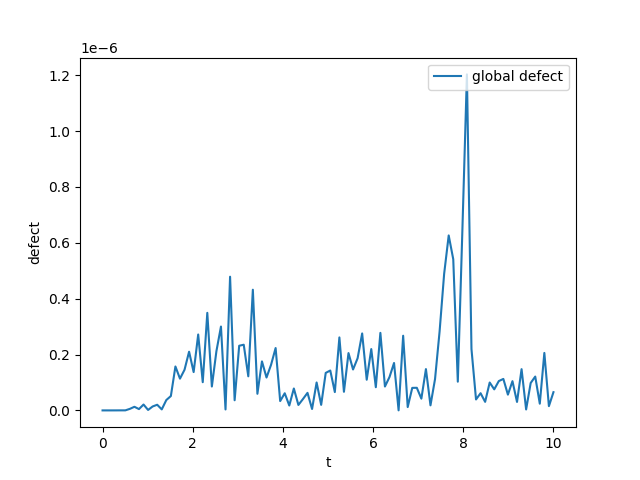
\includegraphics[width=0.7\linewidth]{./figures/rk8_with_hb8_p3_global_defect}
\caption{Defect across the entire domain for RK8 with HB8 on problem 3 at an absolute tolerance of $10^{-6}$.}
\label{fig:rk8_with_hb8_p3_global_defect}
\end{figure}

\begin{figure}[H]
\centering
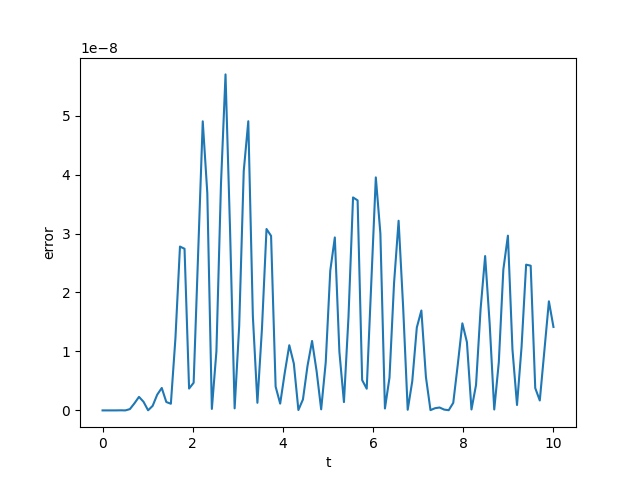
\includegraphics[width=0.7\linewidth]{./figures/rk8_with_hb8_p3_global_error}
\caption{Global Error for RK8 with HB8 on problem 3 at an absolute tolerance of $10^{-6}$.}
\label{fig:rk8_with_hb8_p3_global_error}
\end{figure}

\begin{figure}[H]
\centering
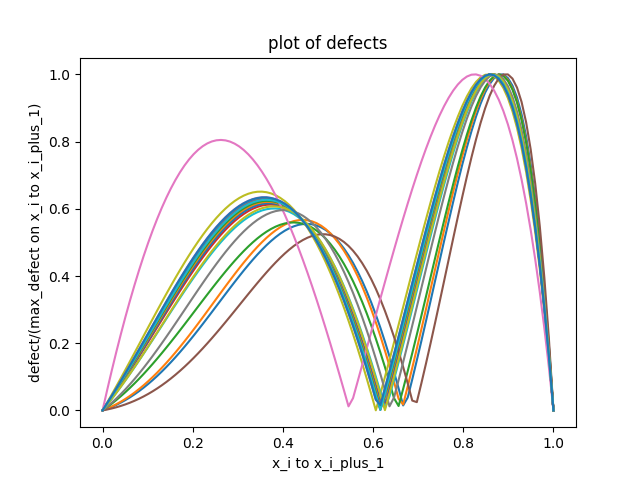
\includegraphics[width=0.7\linewidth]{./figures/rk8_with_hb8_p3_scaled_defects}
\caption{Scaled defects for RK8 with HB8 on problem 3 at an absolute tolerance of $10^{-6}$  mapped onto $[0, 1]$. Despite the noise, the maximum defect mostly appears near $0.8h$.}
\label{fig:rk8_with_hb8_p3_scaled_defects}
\end{figure}

\begin{figure}[H]
\centering
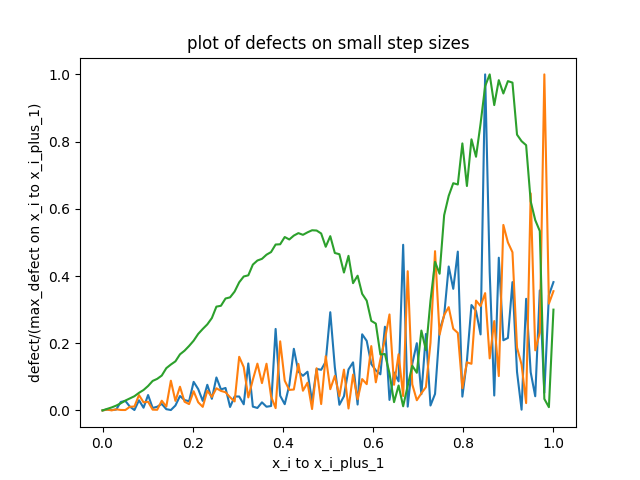
\includegraphics[width=0.7\linewidth]{./figures/rk8_with_hb8_p3_scaled_defects_small_steps}
\caption{Scaled Defects of RK8 with HB8 on small steps on problem 3 at an absolute tolerance of $10^{-6}$ mapped onto $[0, 1]$.}
\label{fig:rk8_with_hb8_p3_scaled_defects_small_steps}
\end{figure}

\begin{table}[h]
\caption {Number of steps taken by RK8 when modified to do defect control with HB8.} \label{tab:rk8_with_hb8_nsteps}
\begin{center}
\begin{tabular}{ c c c } 
Problem & succ. steps & nsteps \\ 
1       & 18             &        19 \\ 
2       & 12             &        15 \\
3       & 24             &        29 \\
\end{tabular}
\end{center}
\end{table}